\begin{figure}[h!]
	
	\centering	
	\tikzset{every picture/.style={line width=0.75pt}} %set default line width to 0.75pt        
	
	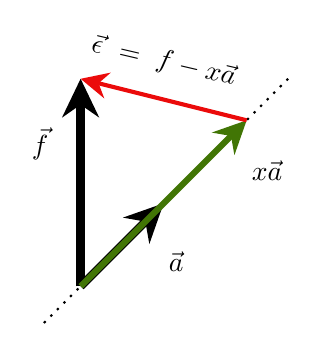
\begin{tikzpicture}[x=0.75pt,y=0.75pt,yscale=-1,xscale=1]
		%uncomment if require: \path (0,300); %set diagram left start at 0, and has height of 300
		
		%Straight Lines [id:da8646407019388729] 
		\draw [line width=3]    (300,160) -- (300,66) ;
		\draw [shift={(300,60)}, rotate = 90] [fill={rgb, 255:red, 0; green, 0; blue, 0 }  ][line width=0.08]  [draw opacity=0] (18.75,-9.01) -- (0,0) -- (18.75,9.01) -- (12.45,0) -- cycle    ;
		%Straight Lines [id:da7219714554771439] 
		\draw [line width=3]    (300,160) -- (335.76,124.24) ;
		\draw [shift={(340,120)}, rotate = 135] [fill={rgb, 255:red, 0; green, 0; blue, 0 }  ][line width=0.08]  [draw opacity=0] (18.75,-9.01) -- (0,0) -- (18.75,9.01) -- (12.45,0) -- cycle    ;
		%Straight Lines [id:da6760457934358763] 
		\draw  [dash pattern={on 0.84pt off 2.51pt}]  (400,60) -- (280,180) ;
		%Straight Lines [id:da46619196099432525] 
		\draw [color={rgb, 255:red, 65; green, 117; blue, 5 }  ,draw opacity=1 ][line width=2.25]    (300,160) -- (376.46,83.54) ;
		\draw [shift={(380,80)}, rotate = 135] [fill={rgb, 255:red, 65; green, 117; blue, 5 }  ,fill opacity=1 ][line width=0.08]  [draw opacity=0] (16.07,-7.72) -- (0,0) -- (16.07,7.72) -- (10.67,0) -- cycle    ;
		%Straight Lines [id:da6028958431173239] 
		\draw [color={rgb, 255:red, 235; green, 11; blue, 11 }  ,draw opacity=1 ][line width=1.5]    (380,80) -- (303.88,60.97) ;
		\draw [shift={(300,60)}, rotate = 14.04] [fill={rgb, 255:red, 235; green, 11; blue, 11 }  ,fill opacity=1 ][line width=0.08]  [draw opacity=0] (13.4,-6.43) -- (0,0) -- (13.4,6.44) -- (8.9,0) -- cycle    ;
		
		% Text Node
		\draw (341,142) node [anchor=north west][inner sep=0.75pt]   [align=left] {$\displaystyle \vec{a}$};
		% Text Node
		\draw (275,82) node [anchor=north west][inner sep=0.75pt]   [align=left] {$\displaystyle \vec{f}$};
		% Text Node
		\draw (381,98) node [anchor=north west][inner sep=0.75pt]   [align=left] {$\displaystyle x\vec{a}$};
		% Text Node
		\draw (305.71,35.87) node [anchor=north west][inner sep=0.75pt]  [rotate=-13.17] [align=left] {$\displaystyle \vec{\epsilon } \ =\ f-x\vec{a}$};		
	\end{tikzpicture}
	\caption{2D illustration of an over determined system}
	\label{fig:Overdetermined2D}
\end{figure}